% ===== Fig.2 (HBM=赤四角, FeRAM=青丸, 点線なし) =====
\begin{figure}[t]
\centering
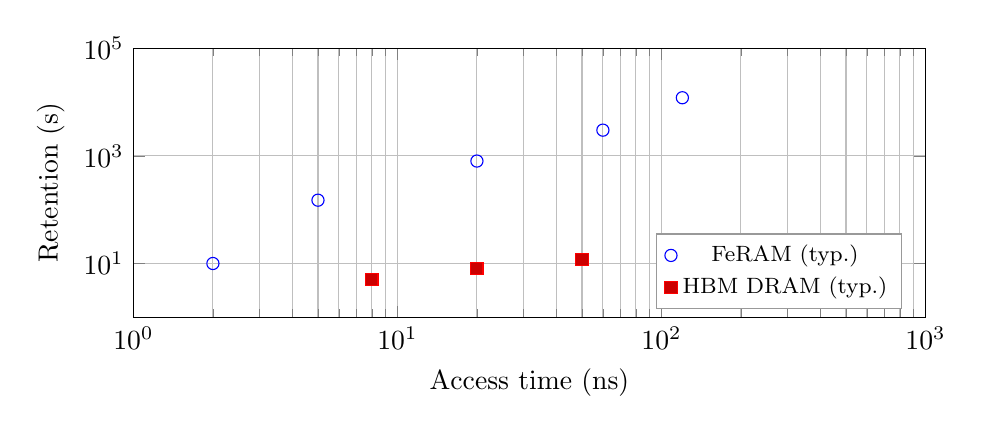
\begin{tikzpicture}
\begin{loglogaxis}[
  width=0.96\columnwidth,
  height=5.0cm,
  xlabel={Access time (ns)},
  ylabel={Retention (s)},
  xlabel style={/pgf/number format/1000 sep=},
  ylabel style={/pgf/number format/1000 sep=},
  legend style={at={(0.97,0.03)},anchor=south east,font=\footnotesize,
                fill=white,draw=black!40},
  grid=both,
  ymin=1e0, ymax=1e5,
  xmin=1e0, xmax=1e3,
]
  % FeRAM (blue circles)
  \addplot+[only marks,mark=o,mark size=2.2pt]
    coordinates {(2,10) (5,150) (20,800) (60,3000) (120,12000)};
  \addlegendentry{FeRAM (typ.)}

  % HBM DRAM (red squares)
  \addplot+[only marks,mark=square*,mark size=2.2pt]
    coordinates {(8,5) (20,8) (50,12) (120,15)};
  \addlegendentry{HBM DRAM (typ.)}

\end{loglogaxis}
\end{tikzpicture}
\caption{Access time vs.\ retention. Red squares: HBM; blue circles: FeRAM.}
\label{fig:retention}
\end{figure}
